\section{Shading}
Once we have found a point of intersection we must now calculate the colour at that point, this will take into account the
reflecance properties of the object and the photon map surrounding it, this will in effect be an evaulation of the rendering
equation, which we will evaluate by spliting the equation into several components, these components are direct illumination,
specular reflection and transmission which we evaluate using raytracing and diffuse interreflection and caustcs which will
use the photon map to estimate the radiance.

Recall from Chapter~\ref{chap:lit}  the rendering equation is given in terms of incoming and outcoming radiance, omitting
emitted radiance we can rewrite the rendering equation with each of the components seperated \cite{JensenBook}

\begin{align*}
L_{r}(x, \omega) =&
			\int_{\Omega}
				f_{r}(x, \omega, \omega')
				L_{i,l}(x,\omega,\omega')
				(\omega \cdot n)d\omega'
			+\\
		&	\int_{\Omega}
				f_{r,S}(x, \omega, \omega')
				(
				L_{i,d}(x,\omega,\omega')
				+
				L_{i,c}(x,\omega,\omega')
				)
				(\omega \cdot n)d\omega'
			+\\
		&	\int_{\Omega}
				f_{r,D}(x, \omega, \omega')
				L_{i,c}(x,\omega,\omega')
				(\omega \cdot n)d\omega'
			+\\
		&	\int_{\Omega}
				f_{r,D}(x, \omega, \omega')
				L_{i,d}(x,\omega,\omega')
				(\omega \cdot n)d\omega'
\end{align*}

where $L_{i,c}$ is the irradiance due to \textbf{LS+D} paths, $L_{i,d}$ due to \textbf{L(S\textbar D)$^+$D} paths and $L_{i,l}$
irradiance directly from light sources (\textbf{LD} paths).

\subsection{Radiance Estimations}
Before we discuss how we utilise the photon map to approximate the global illumination of a scene we must first discuss how
we use the photon map to estimate the radiance at a point. Recall from Section~\ref{chap:lit} the radiance at a point
of intersection can be estimated by,

\begin{equation}
L(x, \omega) = \sum\limits_{n = 1}^N f_r(x,\omega,\omega'_n) \frac{\Delta\Phi_n}{\pi r ^ 2}
\end{equation}

where $f_r(x, \omega,\omega')$ is the BRDF for the surface, we will only use the photon map at diffuse surfaces, as the BRDF
for these surfaces are a constant we can move this calculation out of the summation to give us the following.

\begin{equation}
L(x, \omega) = \frac{\rho_d}{\pi}\sum\limits_{n = 1}^N \frac{\Delta\Phi_n}{\pi r ^ 2}
\end{equation}

It can be seen that we are now estimating the irradiance at the point of intersection, to use the photon map then, we need to
find the N nearest photons to the point at which we are estimating the radiance, to do this we perform the nearest neighbour
algorithm for k-d trees on the photon map.

\begin{algorithm}
\begin{algorithmic}
\caption{K-D tree Nearest Neighbour algorithm}
\State todo
\end{algorithmic}
\end{algorithm}

\subsection{Direct Illumination}
\begin{equation*}
			\int_{\Omega}
				f_{r}(x, \omega, \omega')
				L(x,\omega,\omega')_{i,l}
				(\omega \cdot n)d\omega'
\end{equation*}

Direct illumination is the radiance contribution at a surface directly from the light sources in the scene
(\textbf{LDE} in path notation) this term is responsible for fine details such as shadows in the scene, as a
result we use raytracing to calcualte
the radiance due to direct illumination, it is possible to calculate the radiance due to this term from the photon map but this
approach leads to noise in the final image even when using a high number of photons in the radiance estimate, a comparison of
direct illumination with raytraceing and the photon map can be seen in Figure~\ref{fig:direct_compare} it can be seen that
the illumination calculated by both methods are largly simalar but there is significant variance in the apperance in the
photon mapped image, we can also see that areas close to corners have a lighter apperance, this is due to the use of a
sphere to gather photons in the nearest neighbour search as a result photons that do not belong to a surface are used
as part of the estimate.

\begin{figure}[h]
	\centering
	\begin{subfigure}[c]{0.3\textwidth}
	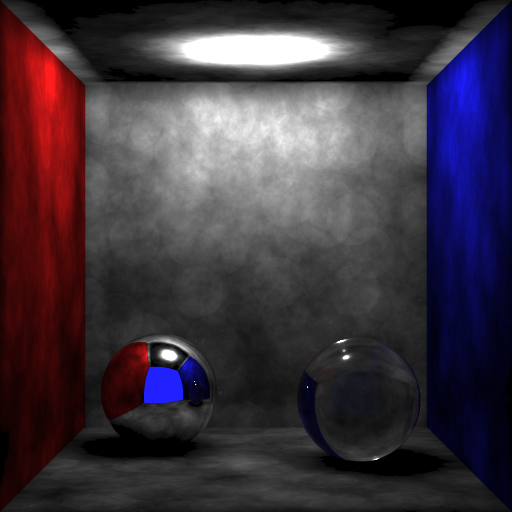
\includegraphics[width=\textwidth]{./images/renders/direct_photon_comp/photon_50000.png}
	\caption{25,000 photons}
	\end{subfigure}
	\begin{subfigure}[c]{0.3\textwidth}
	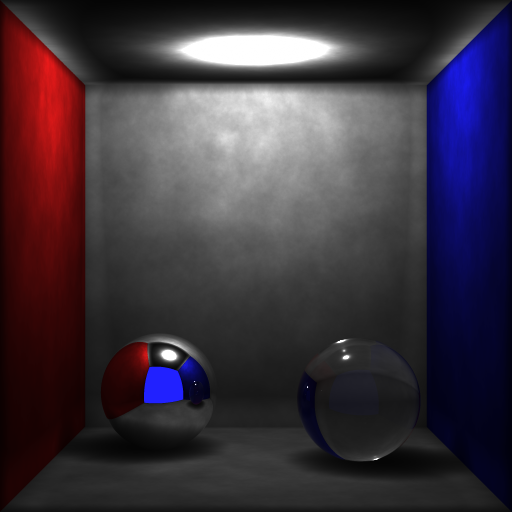
\includegraphics[width=\textwidth]{./images/renders/direct_photon_comp/photon.png}
	\caption{500,000 photons}
	\end{subfigure}
	\begin{subfigure}[c]{0.3\textwidth}
	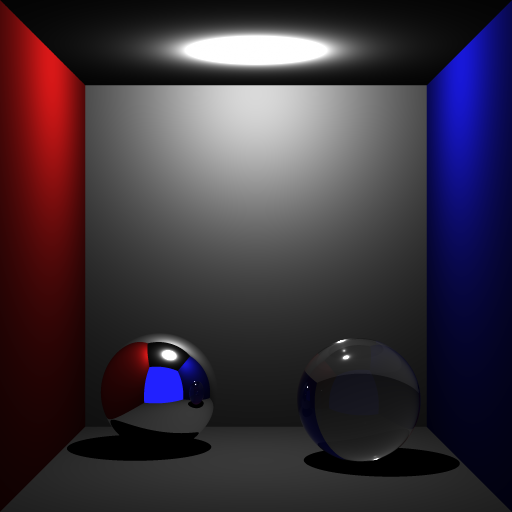
\includegraphics[width=\textwidth]{./images/renders/direct_photon_comp/direct.png}
	\caption{Raytraced}
	\end{subfigure}
	\caption{Comparison of the photon map radiance esitmate with direct illumination}
\label{fig:direct_compare}
\end{figure}

The system currently supports two types of light, point lights and area light, we will first consider calculating the radiance
from a point light as it is the simpler of the two cases.

The radiance from a point light is constant for all points at the same distance from the origin of the light, the radiance at
a point in the scene is given by Equation~\eqref{eq:point_light_radiance}, where the function V is the visibility function, that
is if the point of intersection cannot see the point light it will not contribute the radinace at that point, this will cause
the appearance of shadows in the render.

In the case of area lights calculating the radiance at a point is more complicated, we must calculate the preportion of the
area of the light that is visible at the point of intersection, to do this we sample a number of shadow rays that evaluate the
visibility function across the area of the light.

\begin{figure}
	\centering
	\begin{subfigure}[c]{0.4\textwidth}
	TODO
	\end{subfigure}
	\begin{subfigure}[b]{0.4\textwidth}
		\begin{equation}
		\label{eq:point_light_radiance}
		\centering
			E(x) = \frac
			{
				\Phi_s \cos{\theta}
			}
			{
				4 \pi r^2
			}
		\end{equation}
	\end{subfigure}
\end{figure}

\missingfigure{Area light figure}

\subsubsection{Texture Mapping}
Performing texture mapping requires the ability to query the texture coordinates at a point of intersection, for mesh objects this
will interpolate the barycentric coordinates for the triangle of intersection, spheres use a spherical mapping that uses the
spherical coordinates to generate u,v values, we use linear sampling to calculate the colour from the texture.

\subsection{Specular Reflection and Transmission}
\begin{equation*}
	\int_{\Omega}
	f_{r,S}(x, \omega, \omega')
	(
		L_{i,d}(x,\omega,\omega')
		+
		L_{i,c}(x,\omega,\omega')
	)
	(\omega \cdot n)d\omega'
\end{equation*}
For specular surfaces we again use raytracing to evaluate the contribution, as mentioned previousely the BRDF for specular surfaces
contains two delta functions (one for incoming ray and one for outgoing ray) as a result we cannot use the photon map to evaluate
the contribution from specular surfaces, we will again use raytracing to evaluate this component by tracing an additional reflected
or refracted ray, the equations used to calculate these rays are given in Equations \eqref{eq:refl} and \eqref{eq:refr} where
$\eta_1$ and $\eta_2$ are the refractive index of the medium we are leaving and entering respectivly.

\begin{equation}
\cos{\theta_i} = - \vec{i} \cdot \vec{n}
\qquad\text{and}\qquad
\sin^2\theta_t = \left(\frac{\eta_1}{\eta_2}\right)^2(1 - \cos^2\theta_i)
\end{equation}

\begin{equation}
\vec{r} = \vec{i} + 2 \cos{\theta_i} \vec{n}
\label{eq:refl}
\end{equation}

\begin{equation}
\vec{t} = \frac{\eta_1}{\eta_2} \vec{i} + \left(\frac{\eta_1}{\eta_2} \cos{\theta_i} - \sqrt{1 - \sin^2\theta_t}\right) \vec{n}
\label{eq:refr}
\end{equation}

\begin{figure}
\centering
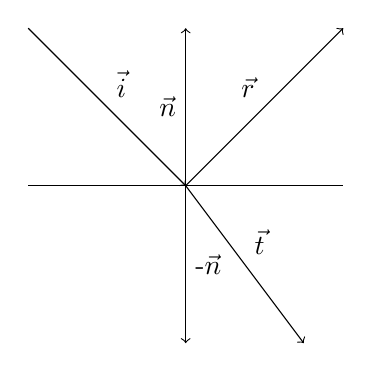
\begin{tikzpicture}[auto]
	\coordinate (m0) at (-2, 0) {};
	\coordinate (m1) at (2, 0) {};

	\coordinate (i) at (0, 0) {};
	\coordinate (n) at (0, 2) {};
	\coordinate (mn) at (0, -2) {};

	\coordinate (inc) at (-2, 2) {};
	\coordinate (refl) at (2,2) {};
	\coordinate (refr) at (1.5, -2) {};

	\draw[-] (m0) to node {} (m1);
	\draw[->] (i) to node {$\vec{n}$} (n);
	\draw[->] (i) to node {-$\vec{n}$} (mn);

	\draw[->] (inc) to node {$\vec{i}$}  (i);
	\draw[->] (i) to node      {$\vec{r}$} (refl);
	\draw[->] (i) to node      {$\vec{t}$} (refr);
\end{tikzpicture}
\end{figure}

\subsubsection{Fresnel Reflection}
Transmissive surfaces reflect a proportion of the radiance incident at the surface as it passes from a material with a different
index of refraction, this proportion is determined by the fresnell equation for dielectrics, which is a function of the refractive
index of the two materials and the incident angle, this is given by equation ~\ref{eq:fresnel}

\begin{equation}
R_f(\theta)
=
\frac{
	\left(
	\frac
	{
	\eta_2 \cos{\theta_i} - \eta_1 \cos{\theta_t}
	}
	{
	\eta_2 \cos{\theta_i} + \eta_1 \cos{\theta_t}
	}
	+
	\frac
	{
	\eta_1 \cos{\theta_i} - \eta_2 \cos{\theta_t}
	}
	{
	\eta_1 \cos{\theta_i} + \eta_2 \cos{\theta_t}
	}
\right)^2
}{2}
\label{eq:fresnel}
\end{equation}

\subsubsection{Schlick Approximation}
Calculating the fresnel term for each refracted ray calculation can be costly, we can howerver use an approximation of the fresnel term
by Schlick \cite{sc94} this is given by:

\begin{equation}
R_s(\theta)=R_0 + \left(1 + R_0\right)\left(1 - \cos\theta\right)^5
\label{eq:schlick}
\end{equation}

where $R_0$ is the fresnel reflectance value for a ray parallel to the surface normal which can be precomputed,
this has been been shown to be up to 30\% faster \cite{deGreve06} than calculating the fresnel term for each refracted ray, Figure~\ref{fig:shlick-compare}
demonstrates the affect of accounting for the fresnell term and also using the Schlick approximation.

As with other aspects of the system where multiple rays can be spawned from a surface interaction (in this case one reflected and one refracted ray)
we use russian roulette in order to determine if we reflect or refract.

\begin{figure}[h]
\centering
\begin{subfigure}[b]{0.3\textwidth}
	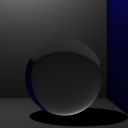
\includegraphics[width=\textwidth]{./images/renders/refraction/no-reflection.png}
	\caption{no Fresnel reflection}
\end{subfigure}
\begin{subfigure}[b]{0.3\textwidth}
	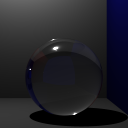
\includegraphics[width=\textwidth]{./images/renders/refraction/fresnel-reflection.png}
	\caption{Fresnel reflection}
\end{subfigure}
\begin{subfigure}[b]{0.3\textwidth}
	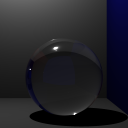
\includegraphics[width=\textwidth]{./images/renders/refraction/render-schlick.png}
	\caption{Schlick reflection}
\end{subfigure}
\caption{Demonstration of Fresnell reflection and the Schlick approximation}
\label{fig:shlick-compare}
\end{figure}

\subsection{Diffuse Interreflection}
\begin{equation*}
		\int_{\Omega}
			f_{r,D}(x, \omega, \omega')
			L_{i,d}(x,\omega,\omega')
			(\omega \cdot n)d\omega'
\end{equation*}

Diffuse interrefection is the contribution that occurs from photons that have been bounced from a diffuse surface at least once
$(\mathbf{LD(S|D)^+E})$ while it is possible to estimate the contribition to the radiance at an intersection point directly from the photon map this
approach can cause visual artifacts due to variance in the estimate in order to reduce these artifacts we perfom a final gather
stage at the point of intersect that produces a diffuse ray that is traced into the scene until a non-specular object is intesected,
we then perform the radiance estimagte at this point and use this information to estimate the radiance incident at the original point of
intersection.  In order for the final gather to produce a correct estimate of the radiance we need to perform this stage multiple times per pixel,
as we are performing distributed raytracing this is a trivial addition.

\begin{figure}
\centering
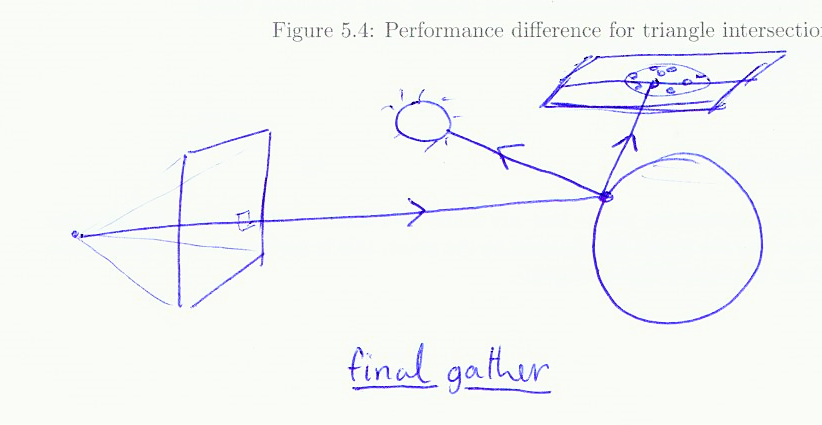
\includegraphics[width=\textwidth]{./images/final_gather.png}
\label{fig:final_gather}
\caption{Final Gather}
\end{figure}

\subsection{Caustics}
\begin{equation*}
		\int_{\Omega}
			f_{r,D}(x, \omega, \omega')
			L_{i,c}(x,\omega,\omega')
			(\omega \cdot n)d\omega'
\end{equation*}

Caustic light occures due to the focusing effect of curved specular surfaces, in other global illumination algorithms
caustics have been hard to simulate \cite{Jensen96a} and often cause large amounts of noise in the final image
with the photon map we are able to estimate the radiance directly from the caustic photon map, as we have seperated the
caustic photons from all other photon paths we reduce the nose that is introduced by caustics in all other radiance
estimates using the photon map. As caustics generally cause sharp visual effects using to few photons in the radiance
estimate can cause unwanted bluring \cite{JensenBook}, in order to reduce this we use a filter as part of the radiance estimate such
that photons near the query point contribute more to the radiance estimate, Jensen suggests the use of one of two filters, the
cone filter and the gaussian filter, each requiring a modification to the photon mapping radiance estimate.

\subsubsection{Cone Filter}
We use the cone filter by applying a weight $w_{pc}$ based upon the distance of the photon from the query point, this will
cause photons that are closer to the point to contribute more to the radiance estimation.

\begin{equation}
w_{pc} = 1 - \frac{d_p}{k r}
\end{equation}

where $k$ is the filter parameter, $d_p$ the distance of the photon from the query point and $r$ the maximum radius of
all photons found in the nearest neighbour search, the updated radiance estimate for the cone fileter is given by:

\begin{equation}
L_r(x, \vec{\omega}) \approx
\frac
{\sum\limits_{p=1}^N f_r(x, \vec{\omega}_p,\vec{\omega})\Delta \Phi_p(x,\vec{\omega}_p)w_{pc}}
{(1 - \frac{2}{3k})\pi r ^2}
\end{equation}

the term $(1 - \frac{2}{3k})$ is a normalisation factor for the cone filter \cite{Foley97}


\begin{figure}[h]

\centering
\begin{subfigure}[b]{0.4\textwidth}
	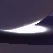
\includegraphics[width=\textwidth]{./images/renders/no-filter.png}
	\caption{without the cone filter}
\end{subfigure}
\begin{subfigure}[b]{0.4\textwidth}
	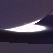
\includegraphics[width=\textwidth]{./images/renders/filter.png}
	\caption{with the cone filter}
\end{subfigure}
\caption{Comparison with and without cone filter}

\end{figure}
